\documentclass{article} % For LaTeX2e
\usepackage{nips14submit_e,times}
\usepackage{hyperref}
\usepackage{url}
\usepackage{amsmath}
\usepackage{graphicx,float,wrapfig}
\usepackage{caption}
\usepackage{subcaption}
\usepackage{natbib}
	\usepackage{bibhacks}
\usepackage[nowarn]{glossaries}
%\documentstyle[nips13submit_09,times,art10]{article} % For LaTeX 2.09

% Use these acronyms instead of writing PMF or Probabilistic Matrix Factorization
% They take care of doing Probabilistic Matrix Factorization (PMF) the first
% time it is mentioned, etc...
\glsdisablehyper
\newacronym{pmf}{PMF}{Probabilistic Matrix Factorization}
\newacronym{lda}{LDA}{Latent Dirichlet Allocation}
\newacronym{bpf}{BPF}{Bayesian Poisson Factorization}
\newacronym{hpf}{HPF}{Hierarchical Poisson Factorization}
\newacronym{cf}{CF}{Collaborative Filtering}
\newacronym{svd}{SVD}{Singular Value Decomposition}
\newacronym{mcmc}{MCMC}{Markov Chain Monte Carlo}
\newacronym{pf}{PF}{Poisson Factorization}

\title{Probabilistic Matrix Factorization}


\author{ 
  Mert Terzihan \\
  Department of Computer Science\\
  Brown University\\
  Providence, RI 02912 \\
  \texttt{mert\_terzihan@brown.edu}
  \And
  Gabriel Barth-Maron \\
  Department of Computer Science \\
  Brown University \\
  Providence, RI 02912 \\
  \texttt{gabriel\_barth-maron@brown.edu}\\
}

% The \author macro works with any number of authors. There are two commands
% used to separate the names and addresses of multiple authors: \And and \AND.
%
% Using \And between authors leaves it to \LaTeX{} to determine where to break
% the lines. Using \AND forces a linebreak at that point. So, if \LaTeX{}
% puts 3 of 4 authors names on the first line, and the last on the second
% line, try using \AND instead of \And before the third author name.

\newcommand{\fix}{\marginpar{FIX}}
\newcommand{\new}{\marginpar{NEW}}

\nipsfinalcopy % Uncomment for camera-ready version

\begin{document}


\maketitle
\begin{abstract}
This is an abstract.
\end{abstract}

\section{Introduction}
\Gls{pmf} is an approximate way to factorize a matrix. In another way, product 
of the matrices that were produced by factorization is an approximation of the 
original matrix. This set of algorithms utilize probabilistic modeling to tackle 
the problem of decomposing matrices. For datasets that are big enough, the 
deterministic methods (i.e \Gls{svd}) could be infeasible to apply. \Gls{pmf} 
models can be learned by EM, \Gls{mcmc}, or as it has been proposed with recent 
research, Variational methods. 

One application of \Gls{pmf} is recommendation systems. Recommendation systems 
aim to produce recommendations to users based on their previous choices and/or 
their demographic information. The interactions between users and items can be 
represented in matrix format, where cell $u,i$ corresponds to the relationship 
between user $u$ and item $i$. The user preferences can be modeled with some 
latent factors. By decomposing the user-item matrix into a product of two 
matrices, we can learn the factors that determine the users' decisions and thus 
cluster users and movies based on these factors. Moreover, artificial 
recommendations can be easily produced with generative models. 

The goal of this paper is to investigate different methods to tackle \Gls{pmf} 
problem especially on movie recommendations, where the interactions between 
users and movies are the ratings that are assigned by users to some movies. Note 
that the corresponding matrix can be sparse, thus making deterministic methods 
inapplicable. The paper is organized as follows: in section 2, we review the 
previous methods that were presented. In section 3, we present an extended 
version of \Gls{lda} model to use ratings as observations instead of bag-of-words 
model. In section 4, we introduce a Gibbs sampler to learn a \Gls{bpf} model. 
The results that have been obtained by learning these two models on 
\textit{MovieLens} dataset, are shared in section 5.

\section{Related Work}

\Gls{pmf} has been used extensively and to success in \gls{cf} systems \cite{koren2009matrix}. Some notable techniques that have been used in this area are: Probabilistic Latent Semantic Analysis (PLSA) \cite{hofmann1999probabilistic}, Multinomial Principal Component Analysis \cite{buntine2002variational}, \acrfull{lda} \cite{lda}, and \acrfull{bpf} \cite{gopalan2013scalable}.

\Gls{lda} is one of the most widely used matrix factorization technique in
\gls{cf} systems. As studied in \cite{lda} and \cite{discrete-pca},
one can observe that LDA is equivalent to factorizing a matrix
probabilistically using a graphical model representation. Instead of dealing with a co-occurence matrix, we will try to propose a model and
a learning algorithm to factorize a matrix where each cell is a rating of an item
by a particular user. Therefore, in addition to LDA, we would also like to generate
ratings that have been assigned by users to each item. 

In \cite{Argwal-fDLA} a method based on LDA is proposed to produce personalized recommendations.
However, fLDA takes into account much more information about the user, i.e. age, 
gender, zipcode, etc. We are going to use a simpler model, which relies on
much less personal information. We will be using only the ratings 
that have been given by the users to specific items.

A LDA-based probabilistic matrix factorization models is proposed in
\cite{conf/icdm/ShanB10}, however instead of using discrete distribution
for generating ratings, it has placed a Gaussian distribution over the user's
ratings. In our investigation we hope to relax this assumption and look into
models that are not necessarily Gaussian.

\acrfull{hpf} \cite{gopalan2013scalable} is a recent \gls{pmf} technique that
extends the Gamma-Poisson (GaP) model proposed by \cite{canny2004gap}.
In addition to \gls{hpf}, the authors of \cite{gopalan2013scalable} also
proposed \gls{bpf}, which sets the rate parameter for the Gamama distributions for
all users and items. It is believed that Poisson factorization better captures
preferences in \gls{cf} tasks. This is proven empirically, as \gls{hpf} and \gls{bpf} perform better than \gls{lda} across a variety of \gls{cf} tasks, including movie recommendation \cite{gopalan2013scalable}.


\section{\acrlong{lda}}
\gls{lda} \cite{lda} is an example of topic models, where a corpus of documents is 
clustered based on the words that each document has. Each document has its own 
topic distribution that might be interpreted as which topic this particular 
document belongs to as a probability vector. Moreover, each topic has a word 
distribution that represents the probability that given a topic, the probability 
of word to occur. For each word in this document, a topic is sampled from the topic 
distribution, and given the topic a word is sampled from the word-topic 
distribution. \gls{lda} is a popular and successful model to cluster documents, 
and we wanted to see if it performs similarly on movie datasets, where ratings 
are produced instead of words. Below is the graphical model for extended 
\gls{lda}: 
\begin{figure}[h]
  \begin{center}
    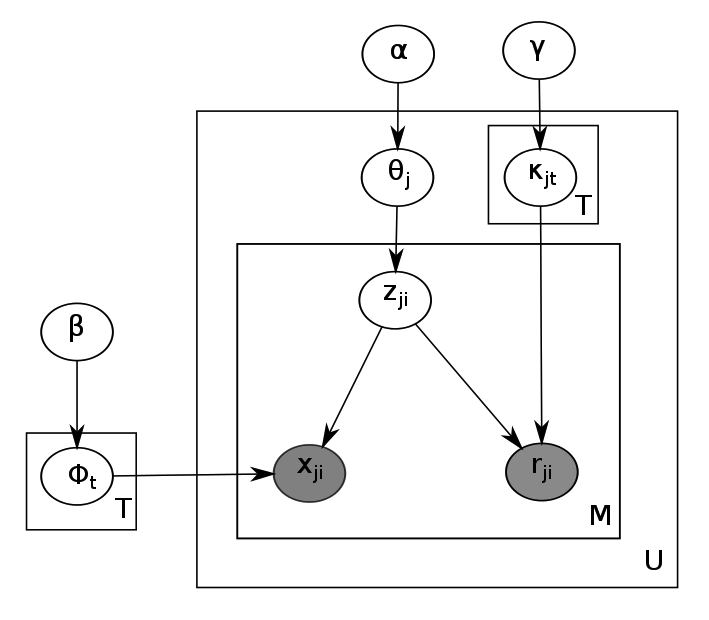
\includegraphics[width=.4\textwidth]{E-LDA.png}
    \caption{Graphical Model for Extended LDA}
    \label{fig:plot1}
  \end{center}
\end{figure}

The random variables follow the below distributions:
\begin{align*}
  &\theta_j \sim Dir(\alpha)\\
  &z_{ji} \sim Cat(\theta_j)\\
  &\phi_t \sim Dir(\beta)\\
  &x_{ji} \sim Cat(\phi_{z_{ji}}) \\
  &\kappa_{jt} \sim Dir(\gamma)\\
  &r_{ji} \sim Cat(\kappa_{z_{ji},j})
\end{align*}

According to the above model, each topic has a distribution over movies ($\phi$) 
and each user has a distribution over topics ($\theta$). For each movie that a 
specific user has rated, a topic ($z_{ji}$) is sampled from $\theta_j$. Using 
this topic, a movie (observed data) is generated as $x_ji$ from topic-movie 
distribution, $\phi$. Until this point, the proposed model is similar to regular 
\gls{lda}. However, we have added a new random variable, $\kappa$, to model the 
ratings that are assigned by users to movies. Every user has a rating 
distribution for each topic. This parameter can be thought as the rating 
preference of the user for the topic. Since our ratings are integers from 1 to 
5, each $\kappa_{jt}$ is a vector of size 5. Following this way, given topic 
assignment for a movie, a rating, $r_{ji}$, can be assigned using $\kappa$. 

\subsection{Collapsed Gibbs Sampler for Extended LDA}

\section{\acrlong{bpf}}
\acrlong{bpf} is a particular model belonging to the more general class of \gls{pf} models. Similar to \gls{lda}, \gls{pf} algorithms are probabilistic models where each item $i$ is represented by $K$ latent topics, and each user $u$ can also be represented by their preferences over these latent topics. In \citep{gopalan2013scalable} two main advantages of the \gls{pf} methods are mentioned. One that is particularly notable is that these methods better capture consumption data, a conjecture that has been reinforced by our own empirical results. To explain this, the authors write that the model can be thought of as allotting a budget to users that they are allowed to spend on items that interest them. Classic \gls{pmf} techniques tend to overestimate the users' overall budget, leading to an overweighting of the zeros.

\subsection{\acrlong{bpf} Model}

\begin{figure}[h]
\begin{center}
	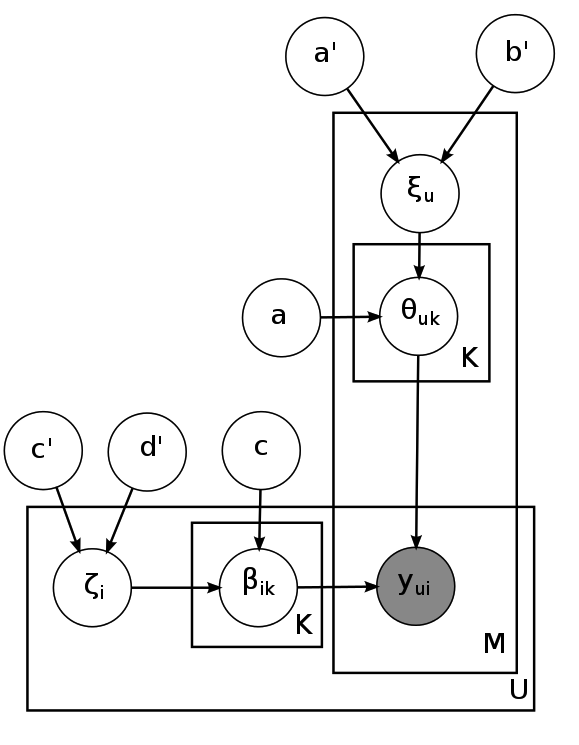
\includegraphics[scale=0.25]{bpf.png}
\end{center}
\caption{\acrlong{bpf} plate diagram}
\label{fig:bpf-model}
\end{figure}

The random variables introduced in Figure \ref{fig:bpf-model} are distributed as follows:
\begin{align*}
	\xi_u &\sim \mathrm{Gamma}\left( a', \frac{a'}{b'} \right) \\
	\theta_{uk} &\sim \mathrm{Gamma}\left( a, \xi_u \right) \\
	\eta_i &\sim \mathrm{Gamma}\left( c', \frac{c'}{d'} \right) \\
	\beta_{ik} &\sim \mathrm{Gamma}\left( c, \eta_i \right) \\
	y_{ui} &\sim \mathrm{Poisson}\left( \theta^\top_u \beta_i \right )
\end{align*}
Where $\xi_u$ is user $u$'s prior over latent topics, $\theta_{uk}$ is user $u$'s preference for topic $k$, $\eta_i$ is item $i$'s prior over latent topics, $\beta_{ik}$ is item $i$'s ``attribute" for topic $k$, and $y_{ui}$ is the distribution over rating for user $u$ and item $i$. The variables $a$, $a'$, $b'$, $c$, $c'$, $d'$, are all fixed hyper-parameters. 

\subsection{Gibbs Sampler for \acrlong{bpf}}
\begin{align*}
	\theta_{uk} \mid \beta, \xi, z, y \sim \mathrm{Gamma}\left(a + \sum_i z_{uik}, \xi_u + \sum_i \beta_{ik} \right)
\end{align*}
\section{Results}

\section{Conclusions}

\section{Future Remarks}

\bibliographystyle{plain}
\bibliography{main}
\end{document}
